%https://tex.stackexchange.com/questions/164991/pgfplots-how-to-fill-bounded-area-under-a-curve-using-addplot-and-fill

%https://tex.stackexchange.com/questions/140312/tikz-shading-region-bounded-by-several-curves
%tikz para graficar areas

%http://latexcolor.com/

%https://www.tablesgenerator.com/
\PassOptionsToPackage{force}{filehook}

\documentclass{beamer}


\usepackage[utf8]{inputenc}
\usepackage{amsmath}
\usepackage{amssymb}% http://ctan.org/pkg/amssymb
\usepackage{amsfonts}
\usepackage{pifont}% http://ctan.org/pkg/pifont
%https://tex.stackexchange.com/questions/42619/x-mark-to-match-checkmark
\newcommand{\cmark}{\ding{51}}
\newcommand{\xmark}{\ding{55}}
%\usepackage{amsfonts}
\usepackage{graphicx} 
\usepackage{subcaption}
\usepackage{hyperref}
\usepackage{cancel}
\usepackage{wrapfig}
\usepackage{enumitem}
\usepackage{comment}
\hypersetup{
	colorlinks=true,
	linkcolor=blue,
	filecolor=magenta,      
	urlcolor=cyan,
}
\newtheorem*{proposicion}{Proposici\'on}
\newtheorem*{teorema}{Teorema}
\renewcommand*{\proofname}{Demostraci\'on}
\newtheorem*{ejercicio}{Ejercicio}
\usepackage{pgf,tikz}
\usetikzlibrary{positioning}
\usetikzlibrary{arrows,patterns}
\usetikzlibrary{arrows.meta}
\usepackage[spanish, activeacute]{babel} %Definir idioma español
\usepackage[utf8]{inputenc} %Codificacion utf-8
\usepackage{multirow}

%   Esconder las soluciones
\newif\ifhideproofs
\hideproofstrue %uncomment to hide proofs

\ifhideproofs
\usepackage{environ}
\NewEnviron{hide}{}
\let\solucion\hide
\let\endsolucion\endhide
\fi

\usepackage{color}
\usepackage{mathpazo}
\usepackage{hyperref}
\usepackage{multimedia}
\usepackage{graphicx}
\usepackage{textcomp}
\usepackage[spanish, activeacute]{babel} 
\usepackage{graphicx} 
\usepackage{booktabs}
\usepackage{cite}
\usepackage{hyperref}
\usepackage{multicol}
\usepackage{multirow,array}

\usepackage{mathrsfs}
%\usepackage{amssymb}

\usepackage{tabularx}
    \newcolumntype{L}{>{\raggedright\arraybackslash}X}
        %\newcolumntype{b}{>{\hsize=1.5\hsize}X}
    %\newcolumntype{s}{>{\hsize=.9\hsize}X}

\usepackage{amsthm}
\newtheorem{thm}{Teorema}
\newtheorem{lem}[thm]{Lema}
\newtheorem{axiom}[thm]{Axioma}
\newtheorem{prop}[thm]{Proposici\'on}
\newtheorem{coro}[thm]{Corolario}
\theoremstyle{definition}
\newtheorem{defn}{Definici\'on}
\DeclareGraphicsExtensions{.pdf,.jpeg,.png,.eps}
\usetheme{CambridgeUS}
\setbeamertemplate{navigation symbols}{}

%Paréntisis y otros
\newcommand{\cmc}{\overset{m.c.}{\rightarrow}}
\newcommand{\p}[1]{\left(#1\right)}
\newcommand{\cor}[1]{\left[#1\right]}
\newcommand{\lla}[1]{\left\{#1\right\}}
\newcommand{\eps}{\varepsilon}
\newcommand{\lol}{\mathcal{L}}
\newcommand{\RR}{\mathbb{R}}
\newcommand{\QQ}{\mathbb{Q}}
\newcommand{\NN}{\mathbb{N}}
\newcommand{\paren}[1]{\left(#1\right)}
\newcommand{\corc}[1]{\left[#1\right]}
\newcommand{\llav}[1]{\left\lbrace#1\right\rbrace}
\newcommand{\partt}[1]{\left(\text{#1}\right)}
\newcommand{\corctt}[1]{\left[\text{#1}\right]}
\newcommand{\llavtt}[1]{\left\lbrace\text{#1}\right\rbrace}
\makeatletter
\def\munderbar#1{\underline{\sbox\tw@{$#1$}\dp\tw@\z@\box\tw@}}
\makeatother

%\usepackage[scr=rsfs,cal=boondox]{mathalfa}
\usepackage[scr=esstix,cal=boondox]{mathalfa}
\usepackage[normalem]{ulem}

% \usepackage{mdframed}
% \newmdtheoremenv{solucion}{Soluci\'on}

% Enmarcar las soluciones
% \newenvironment{solu}
% {%
% \begin{framed}
%   \begin{solucion}
%   }%
%     {%     
%   \end{solucion}
% \end{framed}
% }

%   Esconder las soluciones
\newif\ifhideproofs
%\hideproofstrue %uncomment to hide proofs

\ifhideproofs
\usepackage{environ}
\NewEnviron{hide}{}
\let\solucion\hide
\let\endsolucion\endhide
\fi



%Graficos y cosas
\usepackage{amssymb}
\usepackage{tikz}
\usepackage{pgfplots}
\usepackage{mathtools}
\usepackage{xcolor}
%\pgfplotsset{compat=1.9}
\usepgfplotslibrary{fillbetween,decorations.softclip}
\pgfplotsset{compat = newest}
\usepackage{pst-func}
\usepackage{pstricks}
\usepackage{pst-plot}

% Comando para usar multiples footnotes en un align environment

\makeatletter
\newcommand{\AlignFootnote}[1]{%
    \ifmeasuring@
    \else
        \footnote{#1}%
    \fi
}
\makeatother

%https://tex.stackexchange.com/questions/82782/footnote-in-align-environment


\DeclareGraphicsExtensions{.pdf,.jpeg,.png,.eps}
\usepackage{tikz}
%\usepackage{tikz-cd}
\usetikzlibrary{decorations}
%\usetikzlibrary{snakes}
\usetikzlibrary{cd}

\useoutertheme{split}
\useinnertheme{rounded}


%\beamertemplatenavigationsymbolsempty  %removes navigation bar
\definecolor{rosee}{rgb}{0.7,0.05,0.25}
\definecolor{pacificorange}{cmyk}{0,.6,1,0} %approved Pacific colors 2010
\definecolor{pacificgray}{cmyk}{0,.15,.35,.60}
\definecolor{pacificlgray}{cmyk}{0,0,.2,.4}
\definecolor{pacificcream}{cmyk}{.05,.05,.15,0}
\definecolor{deepyellow}{cmyk}{0,.17,.80,0}
\definecolor{lightblue}{cmyk}{.49,.01,0,0}
\definecolor{lightbrown}{cmyk}{.09,.15,.34,0}
\definecolor{deepviolet}{cmyk}{.79,1,0,.15}
\definecolor{deeporange}{cmyk}{0,.59,1,18}
\definecolor{dustyred}{cmyk}{0,.7,.45,.4}
\definecolor{grassgreen}{RGB}{92,135,39}
\definecolor{pacificblue}{RGB}{59,110,143}
\definecolor{pacificgreen}{cmyk}{.15,0,.45,.30}
\definecolor{deepblue}{cmyk}{1,.57,0,2}
\definecolor{turquoise}{cmyk}{.43,0,.24,0}
\definecolor{gren}{rgb}{0.2,0.8,0.5}
\definecolor{orang}{rgb}{1,0.64,0}
\definecolor{amethyst}{rgb}{0.6, 0.4, 0.8}
\definecolor{dodgerblue}{rgb}{0.12, 0.56, 1.0}
\definecolor{fandango}{rgb}{0.71, 0.2, 0.54}
\definecolor{forestgreen(traditional)}{rgb}{0.0, 0.27, 0.13}
\definecolor{iris}{rgb}{0.35, 0.31, 0.81}
\definecolor{jazzberryjam}{rgb}{0.65, 0.04, 0.37}
\definecolor{mediumjunglegreen}{rgb}{0.11, 0.21, 0.18}
\definecolor{mediumpersianblue}{rgb}{0.0, 0.4, 0.65}
\definecolor{midnightgreen}{rgb}{0.0, 0.29, 0.33}
\definecolor{orangee}{rgb}{1.0, 0.5, 0.0}

% There are many different themes available for Beamer. A comprehensive
% list with examples is given here:
% http://deic.uab.es/~iblanes/beamer_gallery/index_by_theme.html
% You can uncomment the themes below if you would like to use a different
% one:
%\usetheme{AnnArbor} %boca
%\usetheme{Antibes} %azul y gris
%\usetheme{Bergen} %barra who where
%\usetheme{Berkeley} %bordes
%usetheme{Berlin} %blanco y azul
%\usetheme{Boadilla}
%\usetheme{boxes}
\usetheme{CambridgeUS}
%\usetheme{Copenhagen}
%\usetheme{Darmstadt}
%\usetheme{default}
%\usetheme{Frankfurt}
%\usetheme{Goettingen}
%\usetheme{Hannover}
%\usetheme{Luebeck}
%\usetheme{Malmoe}
%\usetheme{Marburg}
%\usetheme{Montpellier}
%\usetheme{PaloAlto}
%\usetheme{Pittsburgh}
%\usetheme{Rochester}
%\usetheme{Singapore}
%\usetheme{Szeged}
%\usetheme{Warsaw}

%\usecolortheme{beaver}
%\usecolortheme{whale}
%\usecolortheme{orchid}
%\usecolortheme{wolverine}
%\usecolortheme[named=pacificblue]{structure} %replaces the blue of Copenhagen with Pacific orange

\definecolor{myNewColorA}{rgb}{0,0,100}
\definecolor{myNewColorB}{rgb}{0,100,100}
\definecolor{myNewColorC}{rgb}{0,200,100}
\definecolor{myNewColorD}{rgb}{0,100,200}

%\setbeamercolor*{palette primary}{bg=myNewColorA, fg = black}
%\setbeamercolor*{palette secondary}{bg=myNewColorB, fg = black}
%\setbeamercolor*{palette tertiary}{bg=myNewColorC, fg = black}
%\setbeamercolor*{palette quaternary}{bg=myNewColorD, fg = black}

\setbeamercolor*{palette primary}{bg=rosee, fg = white}
\setbeamercolor*{palette secondary}{bg=gren, fg = white}
\setbeamercolor*{palette tertiary}{bg=-red!75!, fg = white}
\setbeamercolor*{palette quaternary}{bg=-red!75!, fg = white}

\newtheorem{proposition}{Proposici\'on}
\newcommand{\ton}{\underset{n\to\infty}{\longrightarrow}}
\newcommand{\cp}{\overset{P}{\rightarrow}}
\newcommand{\cw}{\overset{d}{\rightarrow}}

%\expandafter\def\expandafter\insertshorttitle\expandafter{%
 % \insertshorttitle\hfill%
  %\insertframenumber\,/\,\inserttotalframenumber}

%\mode
%<all>

%Para agrandar el espacio entre renglones de las tablas
%https://tex.stackexchange.com/questions/26690/how-to-add-extra-spaces-between-rows-in-tabular-environment
\renewcommand{\arraystretch}{1.5}

\usepackage{color, xcolor}
\definecolor{codegreen}{rgb}{0,0.6,0}
\definecolor{codegray}{rgb}{0.5,0.5,0.5}
\definecolor{codepurple}{rgb}{0.58,0,0.82}
\definecolor{backcolour}{rgb}{0.95,0.95,0.92}

\usepackage{listings}
\lstdefinestyle{mystyle}{
  backgroundcolor=\color{backcolour},   
  commentstyle=\color{codegreen},
  language = R,
  % commentchar=\#,
  keywordstyle=\color{magenta},
  numberstyle=\tiny\color{codegray},
  stringstyle=\color{codepurple},
  basicstyle=\ttfamily\footnotesize,
  breakatwhitespace=false,         
  breaklines=false,                 
  captionpos=b,                    
  frame=single,
  keepspaces=false,
  % numbers=left,                    
  % numbersep=pt,                  
  % columns=flexible,
  stepnumber=1,
  resetmargins=true,
  showspaces=false,                
  showstringspaces=false,
  showtabs=false,                  
  tabsize=1
}
\lstset{style=mystyle}
  



\def\mydate{\leavevmode\hbox{\twodigits\day/\twodigits\month/\the\year}}
\def\twodigits#1{\ifnum#1<10 0\fi\the#1}

\usepackage[final]{pdfpages}

% PARA AGREGAR IMAGEN EN EL FONDO DE LAS SLIDES
\usebackgroundtemplate%
%{%
 %
\includegraphics[width=\paperwidth,height=\pape%rheight]{slides1/fondo.png}%  
%}


\title{\color{black}{Análisis Estadístico}}
\subtitle{\color{rosee}M\'etodo de estimaci\'on de m\'axima verosimilitud\footnote{Basado en las notas de Ezequiel Smucler}}
\institute[]{UTDT}
\medskip
\date[UTDT 2021]{}

\begin{document}
\begin{frame}
  \titlepage
\end{frame}




\begin{frame}{\color{rosee}Introducción}\small
\begin{itemize}
    \item Tanto el método de momentos como el método de máxima verosimilitud nos dan maneras para encontrar estimadores de cualquier parámetro.
\item Ambos métodos producen (en general) estimadores consistentes y asintóticamente normales, es decir, para tama\~nos
    de muestra grandes su distribuci\'on muestral es aproximadamente
    normal (en la mayoría de los casos que veremos en el curso).

%En el tema anterior consideramos el método de momentos como un mecanismo general para construir estimadores para los parámetros de un modelo estadístico.\\
%\medskip
%Aquí estudiaremos otro m\'etodo de estimaci\'on, llamado
%  el m\'etodo de \textbf{m\'axima verosimilitud}. Este m\'etodo tiene propiedades interesantes:\medskip
 % \begin{itemize}
 % \item Resulta más intuitivo que el m\'etodo de
 %   los momentos.\medskip

 % \item Al igual que el método de momentos produce (bajo condiciones generales) estimadores consistentes; y además estos son invariantes:\medskip
  
  %\begin{itemize}
  %    \item Si $\widehat{\theta}_{MV}$ es el estimador de
  %  m\'axima verosimilitud de $\theta$, entonces $g(\widehat{\theta}_{MV})$ es el
  %  estimador de m\'axima verosimilitud de $g(\theta)$ (momentos no
  %  tiene esta propiedad).
  %\end{itemize}
  %\end{itemize}
%\end{frame}

%\begin{frame}{\color{rosee} Introducción}
%  \begin{itemize}
%  \item Bajo condiciones generales, el estimador de m\'axima
  %  verosimilitud es asintóticamente normal, es decir, para tama\~nos
   % de muestra grandes su distribuci\'on muestral es aproximadamente
  %  normal (momentos tiene la misma propiedad).\medskip
 % \item M\'as a\'un la normal est\'a centrada en el par\'ametro
  %  verdadero (momentos tiene la misma propiedad).\medskip
  \item  ¿Por qu\'e querr\'iamos utlizar el método de m\'axima verosimilitud para obtener estimadores de parámetros, si momentos
    es un método tan f\'acil? Veremos que, bajo condiciones generales, la \textbf{varianza asint\'otica}
    del estimador de m\'axima verosimilitud es la m\'inima posible entre
    los estimadores que tienen sesgo que es asintóticamente cero
    (\textbf{el método de momentos no tiene esta propiedad}).
    
    \medskip
  \end{itemize}
  ... empecemos por definir lo que entendemos por (función de) verosimilitud.
\end{frame}

\begin{frame}{\color{rosee} Función de densidad y función de verosimilitud}
\small
  
    Sea $f(x_{1},\dots,x_{n};\theta)$ la funci\'on de densidad de un
    vector aleatorio  $\munderbar{X}=(X_{1},\dots,X_{n})$, que depende de  $\theta$. \underline{La funci\'on de $\theta$} 
    \[L_{n}(\theta)=f(x_{1},\dots,x_{n};\theta),\]
  para \textbf{$\munderbar{x}=x_{1},\dots,x_{n}$ fijos},
    se llama funci\'on de verosimilitud.

  \begin{itemize}
      \item  \textbf{Interpretación:} Si $\munderbar{X}$ es un vector aleatorio \textbf{discreto}, $f(\munderbar{x};\theta)=P_\theta(X_1=x_{1},\dots,X_n=x_{n})$ ``probabilidad de observar una muestra como $\munderbar{x}$ cuando el parámetro del modelo vale $\theta$''.
      \item \textbf{Para el caso discreto} podemos interpretar la función de verosimilitud  $L_n(\theta)$ como la probabilidad de observar la muestra $\munderbar{x}$ para cada posible valor del parámetro $\theta$ en la población. 
    \item \textbf{Para el caso continuo } podemos interpretar la función de verosimilitud  $L_n(\theta)$ como la \sout{probabilidad} verosimilitud de observar la muestra $\munderbar{x}$ para cada posible valor del parámetro $\theta$ en la población porque la función de densidad no es una función de probabilidad puntual.    
  \end{itemize}

  
\end{frame}

\begin{frame}{\color{rosee} $L_n(\theta)$ si $X_i\stackrel{iid}{\sim}$. Ejemplo 1, dados datos $\munderbar{x}$}\small

   Sea $L_{n}(\theta)$ la funci\'on de verosimilitud de una muestra
    \textbf{aleatoria} $X_i\stackrel{iid}{\sim}$ y llamemos $f(x;\theta)$ a la funci\'on
    de densidad que tienen en com\'un las v.a. de dicha muestra, luego Ccmo $X_{1},\dots,X_{n}$ son v.a.i.i.d., su funci\'on de
    densidad conjunta se factoriza:
    \[L_{n}(\theta)= f(x_{1};\theta)f(x_{2};\theta)\dots
    f(x_{n};\theta)\] 

\textbf{En particular,} si $X_i\stackrel{iid}{\sim}Be(p)$, podemos escribir $f(x;p)=p^x(1-p)^{1-x}$ y por lo tanto,
\[L_n(p)=p^{\sum_{i=1}^nX_i}(1-p)^{n-\sum_{i=1}^nX_i}\]
\color{gray}
¿Qué informaci\'on est\'a codificada en $L_n(p)$?  
  
Sea una muestra aleatoria de 10 bicicletas del
    sistema de bicicleta p\'ublicas en CABA. Sea $p=P(\text{bicicleta vandalizada})$ y definamos
    $X_{i}=1$ si la $i-$\'esima bicicleta fue vandalizada y $X_{i}=0$ en
    otro caso. Luego $X_{i}\stackrel{iid}{\sim}Ber(p)$.
     
 Supongamos que en una muestra dada  \[x_1=1,x_2=0,x_3=1,x_4=0,x_5=0,x_6=0,x_7=0,x_8=0,x_9=0,x_{10}=1\]
    y por lo tanto
    \[L_{10}(p)=p^{\sum_{i=1}^{10} x_{i}} (1-p)^{10-\sum_{i=1}^{10}
      x_{i}}=p^{3}(1-p)^{7}\]
  
\end{frame}


%\begin{frame}
%\begin{itemize}
%    \item Ejemplo: Si $X\sim \text{Pois}(\theta)$ y (asumiendo muestreo aleatorio) $X_1=2,X_2=5,X_3=1,X_4=3$; Construye, grafica e interpreta $L_4(\theta)$.\medskip
%    \item ¿Qué ocurre con $L_4(\theta)$ cada vez que se realiza la muestra aleatoria?
%\end{itemize}  
%\begin{figure}
%    \centering
%    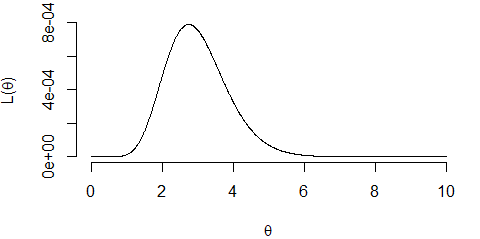
\includegraphics{slides4/img/VerosPoiss.png}
%    \caption{Función de verosimilitud para los datos $X_1=2,X_2=5,X_3=1,X_4=3$. }
%    \label{fig:my_label}
%\end{figure}
%\end{frame}






\begin{frame}{\color{rosee} La verosimilitud $L_{10}(p)$ y la log-verosimilitud $\ln\left(L_{10}(p)\right)$ }
\small Graficamos $L_{10}(p)$ y $\ln\left(L_{10}(p)\right)$. Notemos que el valor de $\theta$ que maximiza ambas funciones el mismo porque $\ln(\cdot)$ es una \textbf{función creciente}.
  % Pablo: gr\'afico de la likelihood y log likelihood tipo figure 7.5
  % del devore.
  
    \begin{figure}
      \centering
      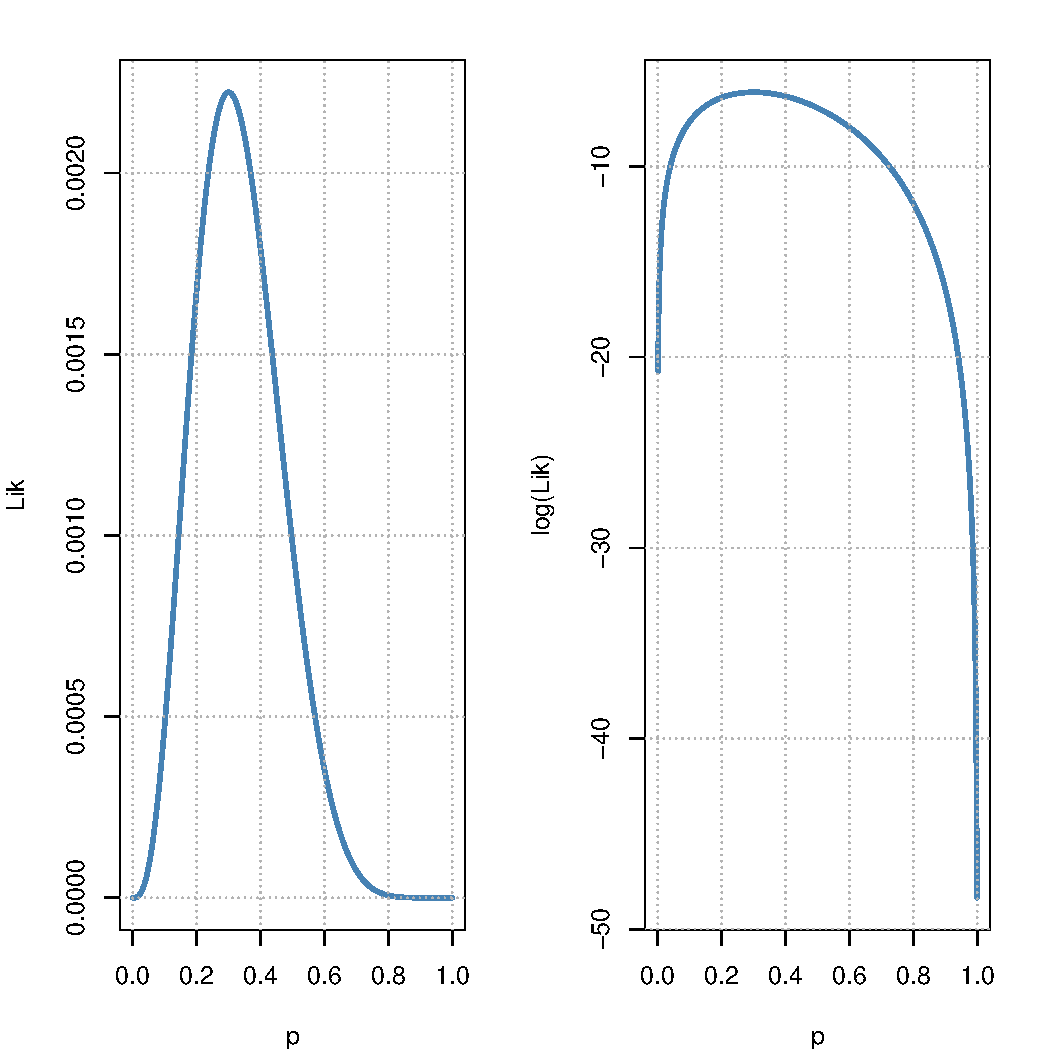
\includegraphics[height=.75\textheight]{img/likelihood.pdf}
    \end{figure}
  
\end{frame}


\begin{frame}{\color{rosee}Ejemplo 1 dados datos de una muestra $\munderbar{x}$}
  \small
    Buscamos $p$ que maximice $\ln(L_{10}({p}))$ para la muestra $\munderbar{x}$. \textbf{Como se
    trata de una funci\'on suave}, para encontrar su m\'aximo, nos
    alcanza con: \textbf{1)} derivar, \textbf{2)} igualar a cero y despejar $p$ y \textbf{3) }chequear que la soluci\'on encontrada sea un m\'aximo (por ejemplo, viendo que la segunda derivada es negativa en la
      soluci\'on).
   \begin{align*}
       \displaystyle\max_{p}\, 3\ln(p)+7\ln(1-p)&\\
       \frac{\partial}{\partial p }\ln(L_{10}({p})) &=
    \frac{3}{p}-\frac{7}{1-p}\\
  \text{CPO}(p):&
    \frac{3}{p^*}-\frac{7}{1-p^*}=0 \Leftrightarrow p^*=\frac{3}{10}
   \end{align*}
    Adem\'as para todo $p$,
    $$
    \frac{\partial^{2}}{\partial p^{2} }\ln(L_{10}({p})) =
    -\frac{3}{p^2}-\frac{7}{(1-p)^{2}}
    <0.
    $$

\end{frame}

\begin{frame}{\color{rosee} La funci\'on de verosimilitud $\mathcal{L}_n(\theta)$}
Si pensamos en la función de verosimilitud ex-ante de que se realice la muestra aleatoria (antes de que $\munderbar{X}=X_1,\dots,X_n$ tomen valores concretos), entonces la función de verosimilitud es una función aleatoria de $\theta$:\medskip
  \begin{alertblock}{Notaci\'on}
    Usaremos la notaci\'on 
    \[\mathcal{L}_{n}(\theta)=f(X_{1};\theta)f(X_{2};\theta)\dots
    f(X_{n};\theta)\]
    es decir, $\mathcal{L}_{n}(\theta)$ es la ``versi\'on aleatoria'' de la
    funci\'on de verosimilitud.
  \end{alertblock}
 \medskip
 \begin{itemize}
     \item Podemos pensar en $L_n(\theta)$ como una ``realización'' de $\mathcal{L}_{n}(\theta)$ cuando nos dan datos $\munderbar{x}$.
 \end{itemize}
  
\end{frame}

\begin{frame}{\color{rosee}Ejemplo 1: Modelo Bernoulli}\small
En general, para una muestra aleatoria $\munderbar{X}$ de tamaño $n$ buscamos maximizar para $X_i\stackrel{iid}{\sim}Be(p)$:\[\ln(\mathcal{L}_n(p))=\color{dodgerblue}\displaystyle\sum_{i=1}^nX_i\color{black}\ln(p)+\color{orang}\left(n-\sum_{i=1}^nX_i\right)\color{black}\ln(1-p)\]
   \begin{align*}
       \displaystyle\max_{p}\, \color{dodgerblue}n\overline{X}_n\color{black}\ln(p)+&\color{orang}n(1-\overline{X}_n)\color{black}\ln(1-p)\\
       \frac{\partial}{\partial p }\ln(\mathcal{L}_{n}({p})) &=
    \frac{\color{dodgerblue}n\overline{X}_n}{p}-\frac{\color{orang}n(1-\overline{X}_n)}{1-p}\\
  \text{CPO}(p):&
    \frac{\color{dodgerblue}n\overline{X}_n}{\widehat{p}_{MV}}-\frac{\color{orang}n(1-\overline{X}_n)}{1-\widehat{p}_{MV}}=0 \Leftrightarrow \widehat{p}_{MV}=\overline{X}_n
   \end{align*}
    Adem\'as, para todo $p$,
    $$
    \frac{\partial^{2}}{\partial p^{2} }\ln(\mathcal{L}_{n}({p})) =
    -\frac{\color{dodgerblue}n\overline{X}_n}{p^2}-\frac{\color{orang}n(1-\overline{X}_n)}{(1-p)^{2}}
    <0.
    $$
  

  
\end{frame}



\begin{frame}{\color{rosee}M\'etodo de m\'axima verosimilitud}
  \small

    Sea $\munderbar{X}$ una muestra aleatoria que tiene funci\'on de
    densidad en com\'un $f(x;\theta)$, para un parámetro $\theta$. El estimador de m\'axima verosimilitud se
    define como el $\widehat{\theta}_{MV}$ que maximiza la verosimilitud
    (aleatoria), es decir que cumple que para todo $\widetilde{\theta}$
    $$
    \mathcal{L}_{n}(\widehat{\theta}_{MV})=f(X_{1};\widehat{\theta}_{MV})\dots
    f(X_{n};\widehat{\theta}_{MV}) \geq
    \mathcal{L}_{n}\left(\widetilde{\theta}\right)=f\left(X_{1};\widetilde{\theta}\right)\dots
    f\left(X_{n};\widetilde{\theta}\right)
    $$

    Para una realizaci\'on de la muestra $x_{1},\dots,x_{n}$, podemos estimar puntualmente a $\theta$ usando la fórmula para $\widehat{\theta}$ y reemplazando los datos aleatorios $X_{i}$ por los datos muestrales $x_{i}$.
  
  \begin{alertblock}{Consejo}
    \textbf{Si bien no es necesario}, casi siempre es m\'as f\'acil maximizar
    $\ln(\mathcal{L}_{n}(\theta))$ que $\mathcal{L}_{n}(\theta)$. Esto
    es porque el logartimo convierte productos en sumas, y las sumas son
    m\'as f\'aciles de derivar que los productos. \textbf{Es muy importante notar que si el soporte de las variables $X_i$ depende de $\theta$ no se podrá aplicar logaritmo a la verosimilitud porque  $\displaystyle\lim_{x\to0^+}\ln(x)=-\infty$.}
  \end{alertblock}
\end{frame}

\begin{frame}{\color{rosee}Ejemplo 2: Modelo Poisson}
\small
    Sea $X_{1},\dots,X_{n}$ una muestra aleatoria con distribuci\'on
    Poisson de par\'ametro $\lambda$. La verosimilitud es
    $$
    \mathcal{L}_{n}(\lambda)=e^{-\lambda n}
    \frac{\lambda^{\sum_{i=1}^{n} X_{i}}}{\prod_{i=1}^{n}X_{i}!}.
    $$
    Luego
    $$
    \ln\left(\mathcal{L}_{n}(\lambda)\right)=-\lambda n +\sum_{i=1}^{n}
    X_{i}\ln(\lambda)-\ln\left(\prod_{i=1}^{n}X_{i}!\right).
    $$
    Es f\'acil ver entonces que el estimador de m\'axima verosimilitud es
    $$
    \widehat{\lambda}_{MV}=\frac{1}{n}\sum\limits_{i=1}^{n}X_{i}.
    $$


    \bigskip $\widehat{\lambda}_{MV}$ es insesgado ya que
    $$
    E\left(\widehat{\lambda}_{MV}
    \right)=E(\overline{X}_{n})=E(X_{1})=\lambda
    $$
   además, por la LGN para $X_i\stackrel{iid}{\sim}$ vale qeu $\widehat{\lambda}_{MV}$ es consistente, ya que 
    $$
    \widehat{\lambda}_{MV} =\overline{X}_{n} \cp E(X_{1})=\lambda.
    $$
  
\end{frame}

% \begin{frame}{\color{rosee}M\'axima verosimilitud: ejemplos}
%   \begin{example}[Poisson]
%     
%     Sabemos adem\'as estimar su error standard (recordar clases pasadas...)
%     $$
%     \frac{S}{\sqrt{n}}
%     $$
%     y hasta sabemos que para tama\~nos de muestra grande, por el TCL y el Lemma de Slutzky
%     $$
%     \widehat{\lambda}_{n} -\lambda \approx N\left(0, \frac{S^{2}}{n}\right).
%     $$
%   \end{example}
% \end{frame}

\begin{frame}{\color{rosee}Ejemplo 3: Modelo Exponencial}
  \small
    Sea $X_{1},\dots,X_{n}$ una muestra aleatoria con distribuci\'on
    exponencial de par\'ametro $\lambda$. La verosimilitud es
    $$
    \mathcal{L}_{n}(\lambda)= \lambda^{n}
    e^{-\lambda{\sum_{i=1}^{n} X_{i}}}
    $$
    Luego
    $$
    \ln\left(\mathcal{L}_{n}(\lambda)\right)=n\ln(\lambda) -\lambda
    \sum_{i=1}^{n}
    X_{i}.
    $$
    Es f\'acil ver entonces que el estimador de m\'axima verosimilitud es
    $$
    \widehat{\lambda}_{MV}=\frac{1}{\overline{X}_{n}}.
    $$
  
  Notemos que este estimador es sesgado pero s\'i es consistente para $\lambda$ usando que por LGN para $X_i\stackrel{iid}{\sim}$, $\overline{X}_{n}\cp E(X)=\frac{1}{\lambda}$ y como $g(x)=\frac{1}{x}$ es una función continua, $\widehat{\lambda}_{MV}=g\left(\overline{X}_{n}\right) \cp g\left(E(X)\right)=\lambda$.
\end{frame}



\begin{frame}{\color{rosee}Propiedad de Invarianza}
  %El estimador de m\'axima verosimilitud tiene la siguiente propiedad
%  \'util.
  \begin{proposition}[Invarianza]
    Sea $X_{1},\dots,X_{n}\stackrel{iid}{\sim} f(x;\theta)$ y $\widehat{\theta}_{MV}$ el estimador de MV de $\theta$. Luego el estimador de MV del parámetro $g(\theta)$ (una función del parámetro en la población) será $\widehat{g(\theta)}_{MV}=g(\widehat{\theta}_{MV})$.
  \end{proposition}
\medskip
  \begin{example}
    Sea $X_{1},\dots, X_{n}\stackrel{iid}{\sim}\text{Be}(p)$, calcular el estimador de m\'axima verosimilitud del parámetro $\psi$ (las odds de probabilidad) definido como:
    \[\psi = g(p) = \frac{p}{1-p}\,.\]
  \end{example}
  \medskip
  \begin{itemize}
      \item Como $\widehat{p}_{MV} = \overline{X}_n$, luego $\widehat{\psi}_{MV}=g( \widehat{p}_{MV}) = \frac{\overline{X}_n}{1-\overline{X}_n}$.
  \end{itemize}
\end{frame}

\begin{frame}{\color{rosee}Ejemplo 4: Modelo uniforme}
  \small
    Sea $X_{1},\dots,X_{n}$ una muestra aleatoria con distribuci\'on
    uniforme en el intervalo $(0,\theta]$. Calculemos el estimador de
    m\'axima verosimilitud de $\theta$. La verosimilitud es
    \[\mathcal{L}_{n}(\theta)=\frac{1}{\theta^{n}}\prod_{i=1}^{n}I_{(0,\theta]}(X_{i}),\]
    que no es derivable como funci\'on de $\theta$ y además \textbf{no podemos aplicar logaritmo} porque la verosimilitud podría valer 0. 

    Notemos que
    $\mathcal{L}_{n}(\theta)$ es positiva siempre que $\theta \geq X_{i}$
    para todo $i=1,\dots,n$, es decir, $\mathcal{L}_{n}(\theta)>0$ siempre que
    $\theta\geq \max\left\{X_{1},\dots,X_{n} \right\}$. 

    \medskip
    
    Adem\'as, si
    $\theta\geq \max\left\{X_{1},\dots,X_{n} \right\}$,
    $\mathcal{L}_{n}(\theta)>0$ es decreciente en $\theta$. Concluimos
    que la verosimilitud se maximiza en
    $\max\left\{X_{1},\dots,X_{n} \right\}$ y por lo tanto el estimador de
    m\'axima verosimilitud es
    \[ \widehat{\theta}_{MV}=\max\left\{X_{1},\dots,X_{n} \right\}.\]
  
\end{frame}

%\begin{frame}{\color{rosee}M\'axima verosimilitud}
%\begin{center}
%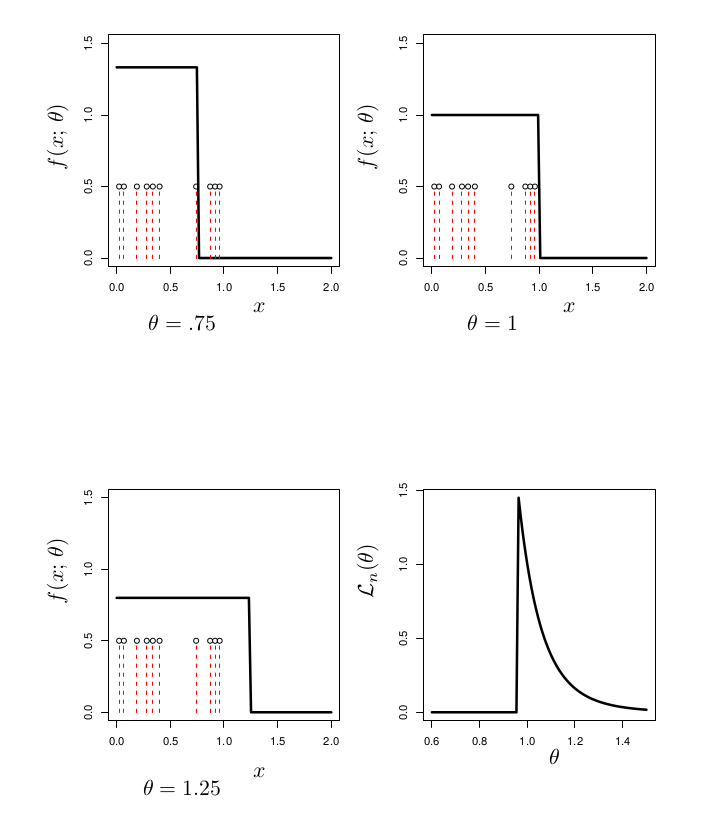
\includegraphics[scale=0.27]{img/lik-unif.png} 
%\end{center}
%\end{frame}


\begin{frame}{\color{rosee}Ejemplo 5: Modelo Laplace}
    Decimos que $X\sim \text{Laplace}(\mu,b)$ si su funci\'on de densidad de $X$ es
    $$
    f(x;\mu,b)=\frac{1}{2b}e^{-\frac{\vert x - \mu\vert}{b}}
    $$
    \begin{figure}
      \centering
      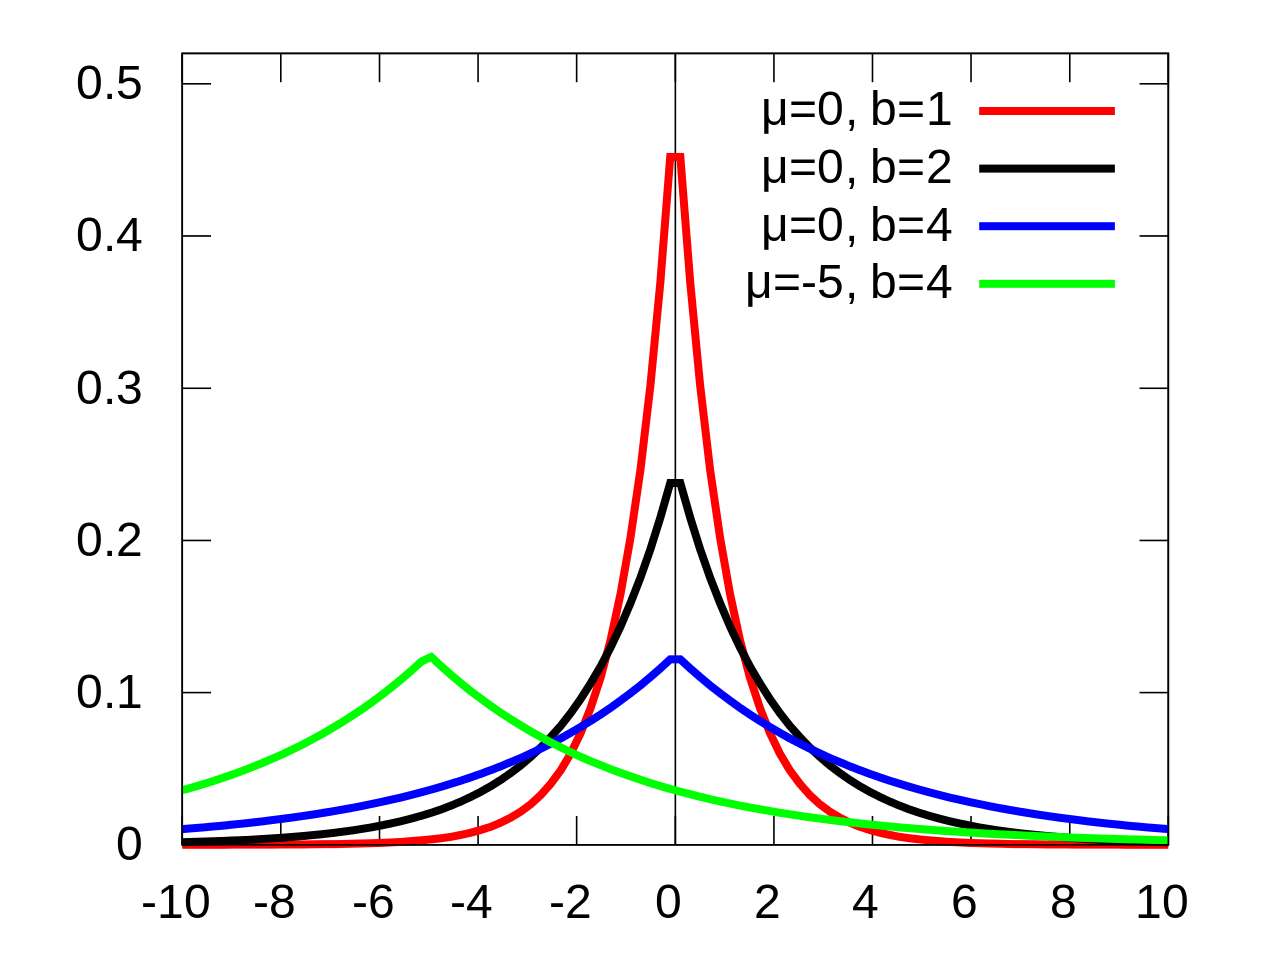
\includegraphics[height=.5\textheight]{img/laplace.png}
      \caption{Densidad del modelo Laplace (el parámetro $b>0$).}
    \end{figure}

\end{frame}

\begin{frame}{\color{rosee}Ejemplo 5: Modelo Laplace}
  \small
    Si $X_{1},\dots,X_{n}\stackrel{iid}{\sim}\text{Laplace}(\theta,1)$, queremos obtener el
    estimador de m\'axima verosimilitud de $\theta$. 
    
    En este ejemplo veremos que $\widehat{\theta}_{MV}=\text{mediana}\{X_1,\cdots, X_n\}$ y se puede demostrar que $\widehat{\theta
    }_{MV} $ estimador es insesgado y consistente para $\theta$ (no lo haremos).
    
    
    \begin{align*}
      \mathcal{L}_{n}(\theta)
      &=(1/2)e^{-\vert X_{1} - \theta\vert}  \dots (1/2)e^{-\vert X_{n} - \theta\vert}
      \\
      &=(1/2^{n}) e^{- \sum_{i=1}^{n}\vert X_{i} - \theta\vert}.
    \end{align*}
    Luego
    $$
    \ln(\mathcal{L}_{n}(\theta))= n \ln(1/2) - \sum_{i=1}^{n}\vert X_{i} - \theta\vert,
    $$
    que no es derivable, ya que el valor absoluto no es derivable en 0.
  
\end{frame}

  
  \begin{frame}{\color{rosee}Ejemplo 5: Modelo Laplace}
\small
Consideremos la funci\'on 
\[sign(x)=\begin{cases}
1  &\text{ si } x>0\\
0 & \text{ si } x=0\\
-1 &\text{ si } x<0\end{cases}\]  
    La derivada de $g(x)=\vert x\vert$ es
    $g^{\prime}(x)=sign(x)$ si $x\neq 0$. Si ``derivamos'', informalmente,
    $\ln(\mathcal{L}_{n}(\theta))$ respecto de $\theta$ e igualamos a
    cero obtenemos
    $$
    \sum_{i=1}^{n} sign\left(X_{i} - \theta\right)=0.
    $$
    Para que esto ocurra, $\theta$ tiene que ser tal que ``la mitad'' de
    los $X_{i}$ tienen que ser menores que $\theta$ y ``la mitad'' sean
    mayores que $\theta$. Si los $X_{i}$ estuvieron ordenados, el
    $\theta$ que resuelve la ecuaci\'on anterior ser\'ia el que est\'a
    en el medio.
  

    La soluci\'on de esta ecuaci\'on es
    $\text{median}(X_{1},\dots,X_{n})$. Es decir
    $$
    \widehat{\theta}_{MV}=\text{mediana}(X_{1},\dots,X_{n}).
    $$
    La derivaci\'on que hicimos no es 100\% formal, pero es
    esencialmente correcta.
  
\end{frame}





\begin{frame}{\color{rosee}Ejemplo 6}
  \small
    Supongamos que tenemos una muestra aleatoria $X_{1},\dots,X_{n}$ tal
    que $X_{i}$ tiene densidad
    $$
    f_{X}(x;\alpha)=\frac{1+\alpha x}{2} I_{[-1,1]}(x)
    $$
    para cierto $\alpha\in [-1, 1]$. Nos interesa estimar $\alpha$. La
    esperanza de $X_{i}$ es $\frac{\alpha}{3}$. El estimador de momentos
    de $\alpha$ es entonces $\widehat{\alpha}_{MM}=3
    \overline{X}_{n}$.
    Es f\'acil ver que $\widehat{\alpha}_{MM}$ es insesgado y
    consistente (por qu\'e?).


    Calculemos ahora el estimador de m\'axima verosimilitud. Tenemos que
    $$
    \mathcal{L}_{n}(\alpha)=\prod_{i=1}^{n} \left(\frac{1+\alpha
        X_{i}}{2}\right)
    $$
    Luego,
    $$
    \ln(\mathcal{L}_{n}(\alpha))=\sum_{i=1}^{n} \ln\left({1+\alpha
        X_{i}}\right) -n\ln(2) .
    $$
Entonces $$\frac{\partial }{\partial \alpha}\ln(\mathcal{L}_{n}(\alpha))=\sum_{i=1}^{n}
    \frac{X_i}{1+\alpha X_{i}}$$
\end{frame}

\begin{frame}{\color{rosee}Ejemplo 6} \small
  
    Tenemos que resolver entonces
    $$
    \sum_{i=1}^{n}
    \frac{X_i}{1+\widehat{\alpha}_{MV} X_{i}}=0.
    $$
El estimador de m\'axima verosimilitud est\'a bien definido como la
    soluci\'on de esta ecuaci\'on, pero no podemos dar una f\'ormula
    cerrada para calcularlo. En estos casos recurrimos a métodos num\'ericos (Newton--Raphson) para aproximar las posibles soluciones de la ecuaci\'on anterior.

    Notemos, no obstante, que el estimador encontrado es un máximo ya que:

    $$\frac{\partial^2 }{\partial \alpha^2}\ln(\mathcal{L}_{n}(\alpha))=-\sum_{i=1}^{n}
    \frac{X_i^2}{(1+\alpha X_{i})^2}<0$$
  
  \begin{alertblock}{\color{rosee}Observaci\'on}
    Habitualmente no existen soluciones cerradas (explícitas) para los estimadores de m\'axima
    verosimilitud. No obstante, se pueden probar propiedades de dichos estimadores.
  \end{alertblock}
\end{frame}



\end{document}

